\state{Curvature of the surface of a sphere~(MCP 25.13)}{
	On the surface of a sphere, such as Earth, introduce spherical polar coordinates in which the metric, written as a line element, takes the form
	\eqn{given4}{
		\dds^2 = a^2 (\ddtht^2 + \sin^2\tht \ddphi^2),
	}
	where $a$ is the sphere's radius.
}

\prob{ \label{4a}
	Show (first by hand and then by computer) that the connection coefficients for the coordinate basis $\{ \pdv*{\tht}, \pdv*{\phi} \}$ are
	\aln{ \label{show4a}
		\Gamtspp &= -\sin\tht \cos\tht, &
		\Gampstp &= \Gampspt = \cot\tht, &
		\text{all others vanish}.
	}
}

\sol{
	We follow the procedure on pp.~1171--1172 of MCP for computing the connection coefficients.  We use (24.38c) to compute
	\eqn{Gamthing}{
		\Gam_{\alp \bet \gam} = \frac{1}{2} (\sg_{\alp \bet, \gam} + \sg_{\alp \gam, \bet} - \sg_{\bet \gam, \alp} + c_{\alp \bet \gam} + c_{\alp \gam \bet} - c_{\bet \gam \alp}),
	}
	where we know the commutation coefficients $c_{\alp \bet \gam}$ vanish in a coordinate basis~\cite[p.~1171]{MCP}.  We raise the first index using (24.38d),
	\eqn{Gamraise}{
		\fv{\Gam}{\mu}{\bet \gam} = \sg^{\mu \alp} \Gam_{\alp \bet \gam}.
	}
	According to MCP~(24.7), the invariant interval is defined
	\eq{
		\dds^2 = \sg_{\alp \bet} \Del x^\alp \Del x^\bet.
	}
	This means the metric tensor components can be read off of Eq.~\refeq{given4} as
	\aln{ \label{met4}
		\sgstt &= a^2, &
		\sgspp &= a^2 \sin^2\tht.
	}
	The only nonzero derivative is
	\eq{
		\sg_{\phi \phi, \tht} = 2 a^2 \sin\tht \cos\tht.
	}
	so only connection coefficients with some combination of $\{ \phi, \phi, \tht \}$ can be nonzero.  Applying Eq.~\refeq{Gamthing} to the possible candidates, we find
	\al{
		\Gam_{\tht \phi \phi} &= \frac{1}{2} (\sg_{\tht \phi, \phi} + \sg_{\tht \phi, \phi} - \sg_{\phi \phi, \tht}) = -a^2 \sin\tht \cos\tht, \\
		\Gam_{\phi \tht \phi} &= \frac{1}{2} (\sg_{\phi \tht, \phi} + \sg_{\phi \phi, \tht} - \sg_{\tht \phi, \tht}) = a^2 \sin\tht \cos\tht, \\
		\Gam_{\phi \phi \tht} &= \frac{1}{2} (\sg_{\phi \phi, \tht} + \sg_{\phi \tht, \phi} - \sg_{\phi \tht, \phi}) = a^2 \sin\tht \cos\tht.
	}
	The components of the inverse metric tensor are
	\al{
		\sgtt &= \frac{1}{a^2}, &
		\sgpp &= \frac{1}{a^2 \sin^2\tht}.
	}
	Now applying Eq.~\refeq{Gamraise}, we have
	\ans{\al{
		\Gamtspp &= \sgtt \Gam_{\tht \phi \phi} = -\sin\tht \cos\tht, &
		\Gampstp &= \sgpp \Gam_{\phi \tht \phi} = \cot\tht, &
		\Gampspt &= \sgpp \Gam_{\phi \phi \tht} = \cot\tht.
	}}%
	as we wanted to show. \qed
	
	By computer, we use a Mathematica notebook adapted from Ref.~\cite{Hartle}:
	
	\scalebox{0.625}{
		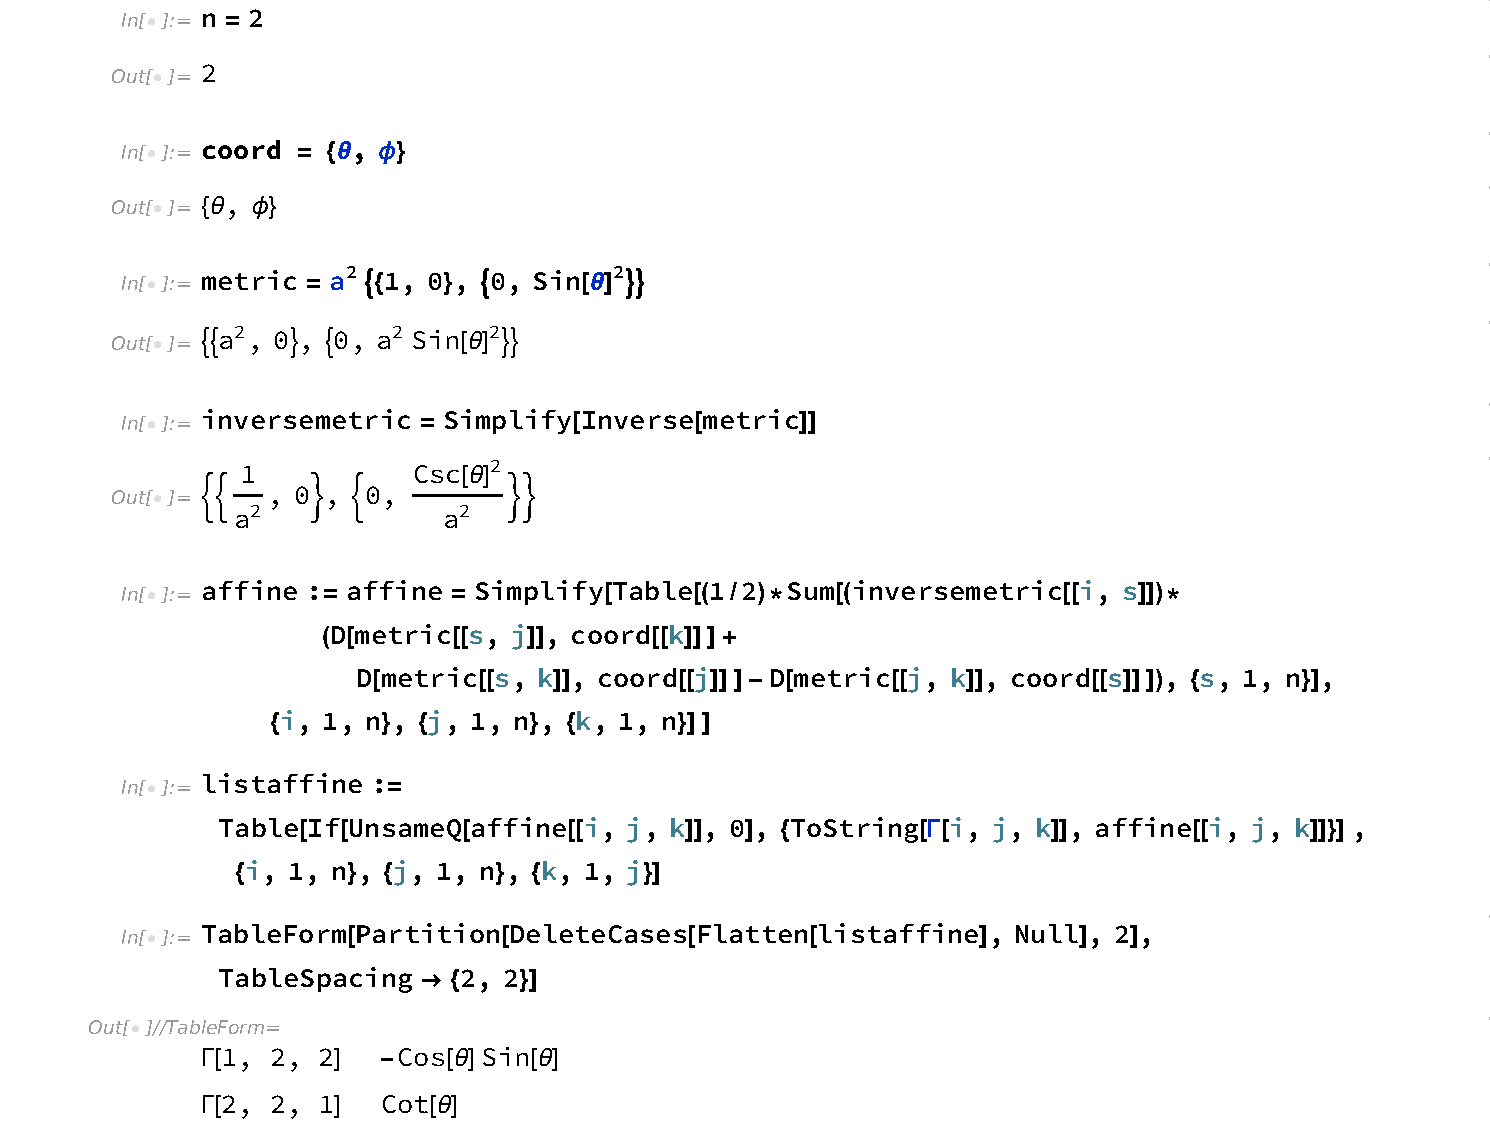
\includegraphics{4a}
	}
	
	Here $\tht \to 1$ and $\phi \to 2$.  Taking into account that in a coordinate basis $\Gam_{\alp \bet \gam}$ is symmetric in its last two indices~\cite[p.~1172]{MCP}, these match our result.
}



\prob{
	Show that the symmetries (25.45) of the Riemann tensor guarantee that its only nonzero components in the above coordinate basis are
	\eq{
		\Rstptp = \Rsptpt = -\Rstppt = -\Rspttp.
	}
}

\sol{
	According to MCP~(25.45a),
	\aln{ \label{symm}
		R_{\alp \bet \gam \del} &= -R_{\bet \alp \gam \del}, &
		R_{\alp \bet \gam \del} &= -R_{\alp \bet \del \gam}, &
		R_{\alp \bet \gam \del} &= +R_{\gam \del \alp \bet}.
	}
	Applying these to the six possible permutations of $\{ \tht, \tht, \phi, \phi \}$, we have
	\ans{\al{
		R_{\tht \tht \phi \phi} &= -R_{\tht \tht \phi \phi} = 0, &
		R_{\phi \phi \tht \tht} &= -R_{\phi \phi \tht \tht} = 0, &
		R_{\tht \phi \phi \tht} &= -R_{\phi \tht \phi \tht} = -R_{\tht \phi \tht \phi} = R_{\phi \tht \tht \phi},
	}}%
	as we wanted to show. \qed
}



\prob{
	Show, first by hand and then by computer, that
	\eq{
		\Rstptp = a^2 \sin^2\tht.
	}
}

\sol{
	From Eq.~\refeq{show2},
	\eq{
		\fv{R}{\tht}{\phi \tht \phi} = \fv{\Gam}{\tht}{\phi \phi, \tht} - \fv{\Gam}{\tht}{\phi \tht, \phi} + \fv{\Gam}{\tht}{\mu \tht} \fv{\Gam}{\mu}{\phi \phi} - \fv{\Gam}{\tht}{\mu \phi} \fv{\Gam}{\mu}{\phi \tht} - \fv{\Gam}{\tht}{\phi \mu} \sfv{c}{\tht \phi}{\mu}.
	}
	From Eq.~\refeq{show4a},
	\al{
		\fv{\Gam}{\tht}{\phi \phi, \tht} &= \sin^2\tht - \cos^2\tht, &
		\fv{\Gam}{\phi}{\tht \phi, \tht} &= \fv{\Gam}{\phi}{\phi \tht, \tht} = -\csc^2\tht, &
		\fv{\Gam}{\tht}{\phi \phi, \phi} &= \fv{\Gam}{\phi}{\tht \phi, \phi} = \fv{\Gam}{\phi}{\phi \tht, \phi} = 0.
	}
	We also know that all $c_{\alp \bet \gam} = 0$.  Equation~\refeq{thing4c} is then
	\eq{
		\fv{R}{\tht}{\phi \tht \phi} = \fv{\Gam}{\tht}{\phi \phi, \tht} - \fv{\Gam}{\tht}{\phi \phi} \fv{\Gam}{\phi}{\phi \tht}
		= \sin^2\tht - \cos^2\tht - (-\sin\tht \cos\tht) (\cot\tht)
		= \sin^2\tht.
	}
	Lowering the first index using Eq.~\refeq{met4}, we find
	\eq{
		\ans{ \Rstptp = \sgstt \fv{R}{\tht}{\phi \tht \phi}
		= a^2 \sin^2\tht }
	}
	as we wanted to show. \qed
	
	Continuing the notebook from \ref{4a},
	
	\scalebox{0.625}{
		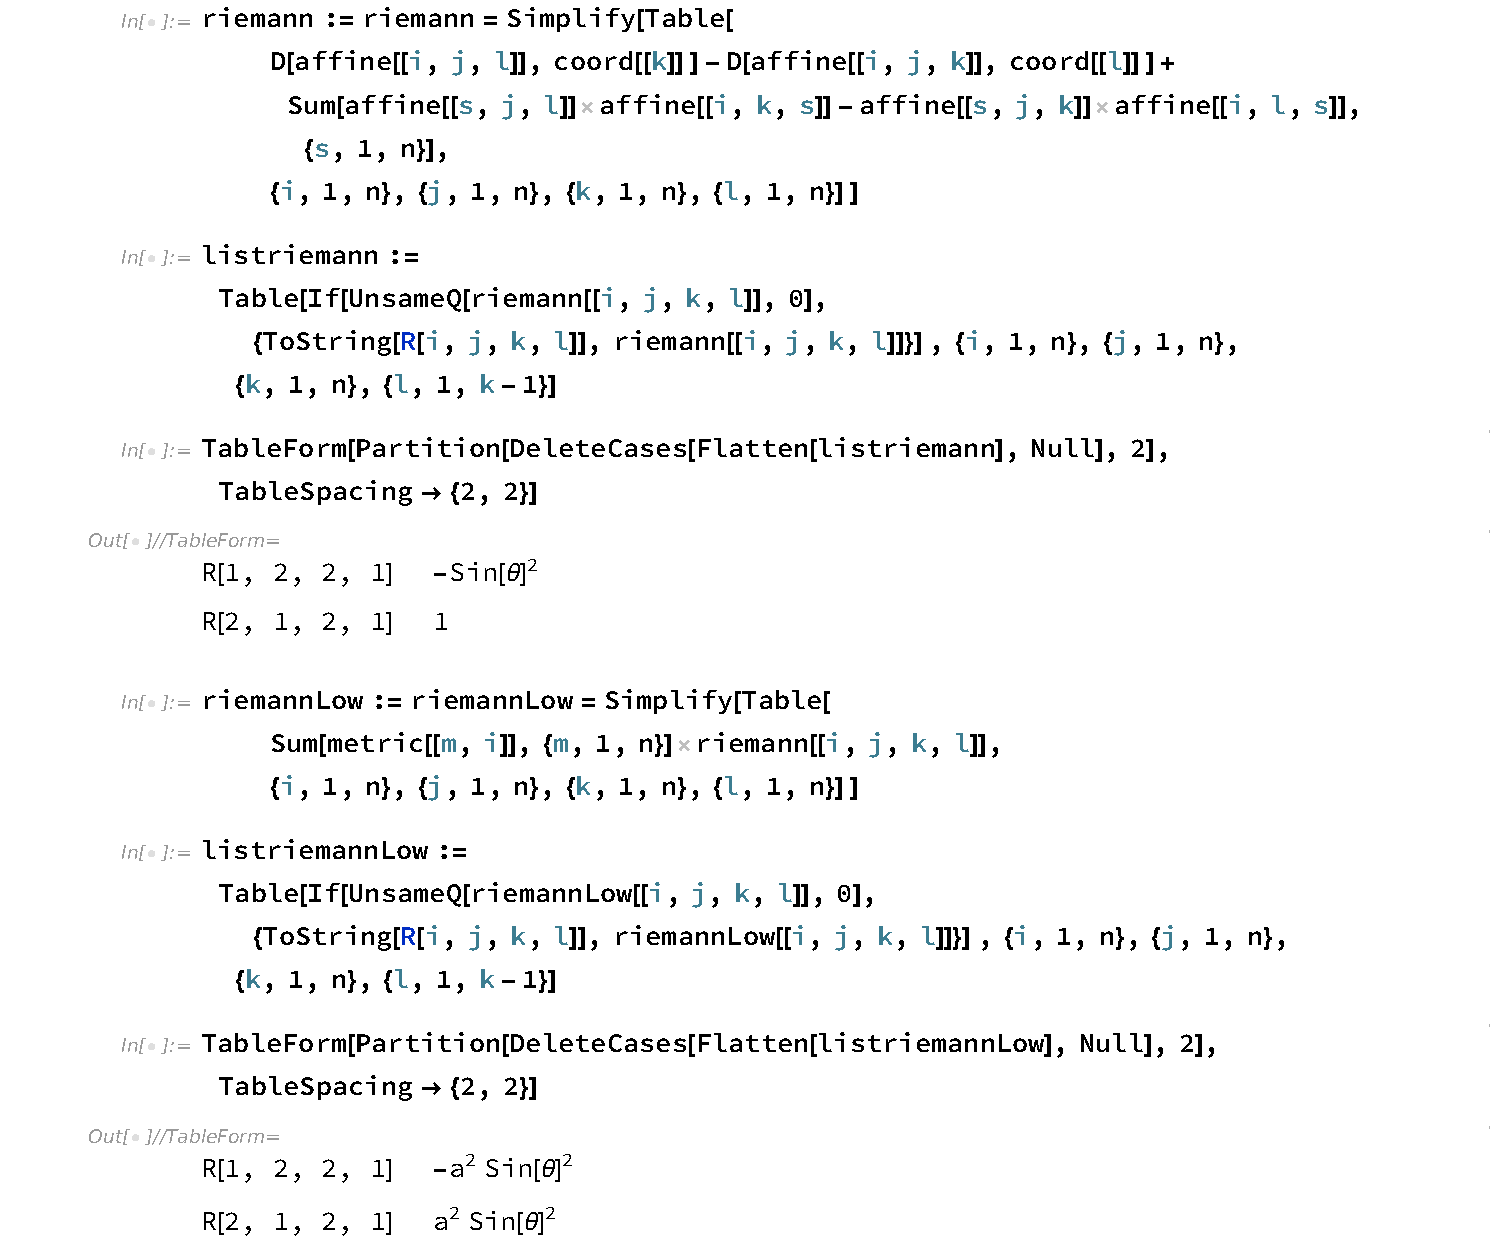
\includegraphics{4c}
	}
	
	Here the second list of \nolinkurl{R[_, _, _, _]} has the first index lowered.  By Eq.~\refeq{symm}, \nolinkurl{R[1, 2, 2, 1]} is equivalent to $\text{\nolinkurl{R[1, 2, 1, 2]}} = \Rstptp$, which agrees with our calculation.
}



\prob{
	Show that in the basis
	\eqn{basis}{
		\{ \vesthh, \vesphh \} = \curly{ \frac{1}{a} \pdv{\tht}, \frac{1}{a \sin\tht} \pdv{\phi} },
	}
	the components of the metric, the Riemann tensor, the Ricci tensor, the curvature scalar, and the Weyl tensor are
	\aln{ \label{show4d}
		\sgsjhkh &= \delsjk, &
		\Rsthphthph &= \frac{1}{a^2}, &
		\Rsjhkh &= \frac{1}{a^2} \sgsjhkh, &
		R &= \frac{2}{a^2}, % &
%		\Csthphthph &= 0,
	}
	respectively.  The first of these implies that the basis is orthonormal; the rest imply that the curvature is independent of location on the sphere, as it should be by spherical symmetry.
}

\sol{
	To find the components of the metric, we use MCP~(24.16),
	\eq{
		\dds^2 = \sg_{\alp \bet} \dd{x^\alp} \dd{x^\bet}.
	}
	Comparing this with Eq.~\refeq{given4}, we have
	\eq{
		\dds^2 = a^2 \ddtht^2 + a^2 \sin^2\tht \ddphi^2
		= \sg_{\thh \thh} \dd{\thh}^2 + \sg_{\phh \phh} \dd{\phh}^2
	}
	since $\dd{\thh} = a \ddtht$ and $\dd{\phh} = a \sin\tht \ddphi$ from Eq.~\refeq{basis}.  We conclude from the above that
	\ans{ \al{
		\sg_{\thh \thh} &= \sg_{\phh \phh} = 1, &
		\sg_{\thh \phh} &= \sg_{\phh \thh} = 0;
	}}%
	that is, $\sgsjhkh = \delsjk$. \qed
	
	To find $\Rsthphthph$, we can adapt the connection coefficients from Problem~1(a) of Homework~3; we simply ignore the coefficients with indices $\hat{r}$ and let $r \to a$ in the ones that remain.  So the only nonzero coefficients are
	\eqn{Gammas}{
		\Gam_{\phh \thh \phh} = -\Gam_{\thh \phh \phh} = \frac{\cot\tht}{a}.
	}
	From Eq.~\refeq{show2},
	\al{
		R_{\thh \phh \thh \phh} &= \sg_{\thh \mu} \fv{R}{\mu}{\phh \thh \phh} \\
		&= \Gam_{\thh \phh \phh, \thh} - \Gam_{\tht \phh \thh, \phh} + \Gam_{\thh \mu \thh} \fv{\Gam}{\mu}{\phh \phh} - \Gam_{\thh \mu \phh} \fv{\Gam}{\mu}{\phh \thh} - \Gam_{\thh \phh \mu} \sfv{c}{\thh \phh}{\mu} \\
		&= \Gam_{\thh \phh \phh, \thh} - \Gam_{\thh \phh \phh} \sfv{c}{\thh \phh}{\phh} \\
		&= \frac{1}{a} \dv{\tht}{\Gam_{\thh \phh \phh}} + \frac{\cot\tht}{a} \Gam_{\thh \phh \phh} \\
		&= \frac{1}{a} \dv{\tht}( -\frac{\cot\tht}{a} ) - \frac{\cot\tht}{a} \frac{\cot\tht}{a} \\
		&= \frac{\csc^2\tht - \cot^2\tht}{a^2} \\
		&= \ans{ \frac{1}{a^2}, }
	}
	where we have used $\sfv{c}{\thh \phh}{\phh} = -\cot\tht / a$ from Problem~1(a) of Homework~3. \qed
	
	It is also useful to note that
	\al{
		R_{\alp \bet \gam \del} = \Gam_{\alp \bet \del, \gam} - \Gam_{\alp \bet \gam, \del} + \Gam_{\alp \mu \gam} \fv{\Gam}{\mu}{\bet \del} - \Gam_{\alp \mu \del} \fv{\Gam}{\mu}{\bet \gam} - \Gam_{\alp \bet \mu} \sfv{c}{\gam \del}{\mu},
	}
	\al{
		R_{\thh \thh \thh \thh} &= \Gam_{\thh \thh \thh, \thh} - \Gam_{\thh \thh \thh, \thh} + \Gam_{\thh \mu \thh} \fv{\Gam}{\mu}{\thh \thh} - \Gam_{\thh \mu \thh} \fv{\Gam}{\mu}{\thh \thh} - \Gam_{\thh \thh \mu} \sfv{c}{\thh \thh}{\mu} = 0, \\
		%
		R_{\phh \phh \phh \phh} &= \Gam_{\phh \phh \phh, \phh} - \Gam_{\phh \phh \phh, \phh} + \Gam_{\phh \mu \phh} \fv{\Gam}{\mu}{\phh \phh} - \Gam_{\phh \mu \phh} \fv{\Gam}{\mu}{\phh \phh} - \Gam_{\phh \phh \mu} \sfv{c}{\phh \phh}{\mu} = 0, \\
		%
		R_{\phh \thh \thh \thh} &= \Gam_{\phh \thh \thh, \thh} - \Gam_{\phh \thh \thh, \thh} + \Gam_{\phh \mu \thh} \fv{\Gam}{\mu}{\thh \thh} - \Gam_{\phh \mu \thh} \fv{\Gam}{\mu}{\thh \thh} - \Gam_{\phh \thh \mu} \sfv{c}{\thh \thh}{\mu}
		= R_{\thh \thh \thh \phh} = 0, \\
		%
		R_{\thh \phh \phh \phh} &= \Gam_{\thh \phh \phh, \phh} - \Gam_{\thh \phh \phh, \phh} + \Gam_{\thh \mu \phh} \fv{\Gam}{\mu}{\phh \phh} - \Gam_{\thh \mu \phh} \fv{\Gam}{\mu}{\phh \phh} - \Gam_{\thh \phh \mu} \sfv{c}{\phh \phh}{\mu}
		= R_{\phh \thh \phh \phh} = 0, \\
		%
		R_{\thh \phh \thh \phh} &= R_{\phh \thh \phh \thh} = \frac{1}{a^2},
	}
	where we have used $\sfv{c}{\thh \thh}{\phh} = \sfv{c}{\phh \phh}{\phh} = 0$ from Problem~1(a) of Homework~3.  From MCP~(25.46),
	\eq{
		\Rsjhkh = \fv{R}{\mu}{\jh \mu \kh}
		= \fv{R}{\thh}{\jh \thh \kh} + \fv{R}{\phh}{\jh \phh \kh}.
	}
	Then
	\al{
		R_{\thh \thh} &= \fv{R}{\mu}{\thh \mu \thh}
		= \fv{R}{\thh}{\thh \thh \thh} + \fv{R}{\phh}{\thh \phh \thh}
		= \frac{1}{a^2}, \\
		%
		R_{\thh \phh} &= \fv{R}{\mu}{\thh \mu \phh}
		= \fv{R}{\thh}{\thh \thh \phh} + \fv{R}{\phh}{\thh \phh \phh}
		= 0, \\
		%
		R_{\phh \thh} &= R_{\thh \phh}
		= 0, \\
		%
		R_{\phh \phh} &= \fv{R}{\mu}{\phh \mu \phh}
		= \fv{R}{\thh}{\phh \thh \phh} + \fv{R}{\phh}{\phh \phh \phh}
		= \frac{1}{a^2},
	}
	where we have applied MCP~(25.47), $R_{\alp \bet} = R_{\bet \alp}$.  Summarizing these results, we have \ans{$\Rsjhkh = \sgsjhkh / a^2$} as we wanted to show. \qed
	
	From MCP~(25.49), $R = \fv{R}{\alp}{\alp}$.  Then
	\eq{
		R = R_{\tht \tht} + R_{\phh \phh}
		= \frac{1}{a^2} + \frac{1}{a^2}
		= \ans{ \frac{2}{a^2} }
	}
	as desired. \qed
%	
%	From Eq.~\refeq{lowC} and our previous results here,
%	\al{
%		C_{\thh \phh \thh \phh} &= R_{\thh \phh \thh \phh} - \frac{1}{2} \paren{ \sg_{\thh \thh} R_{\phh \phh} - \sg_{\thh \phh} R_{\phh \thh} - \sg_{\phh \thh} R_{\thh \phh} + \sg_{\phh \phh} R_{\thh \thh} } + \frac{1}{12} \paren{ \sg_{\thh \thh} \sg_{\phh \phh} - \sg_{\thh \phh} \sg_{\phh \thh} - \sg_{\phh \thh} \sg_{\thh \phh} + \sg_{\phh \phh} \sg_{\thh \thh} } R \\
%		&= R_{\thh \phh \thh \phh} - \frac{1}{2} \paren{ R_{\phh \phh} + R_{\thh \thh} } + \frac{1}{12} \paren{ 1 + 1 } R \\
%		&= \frac{1}{a^2} - \frac{1}{2} \paren{ \frac{1}{a^2} + \frac{1}{a^2} } + \frac{4}{12} \frac{1}{a^2} \\
%		&= \paren{ 1 - 1 + \frac{1}{3} } \frac{1}{a^2} \\
%		&= \frac{1}{3 a^2}
%	}
%	\hl{which is not correct!!!}
}